\begin{figure}[htpb]
    \centering
    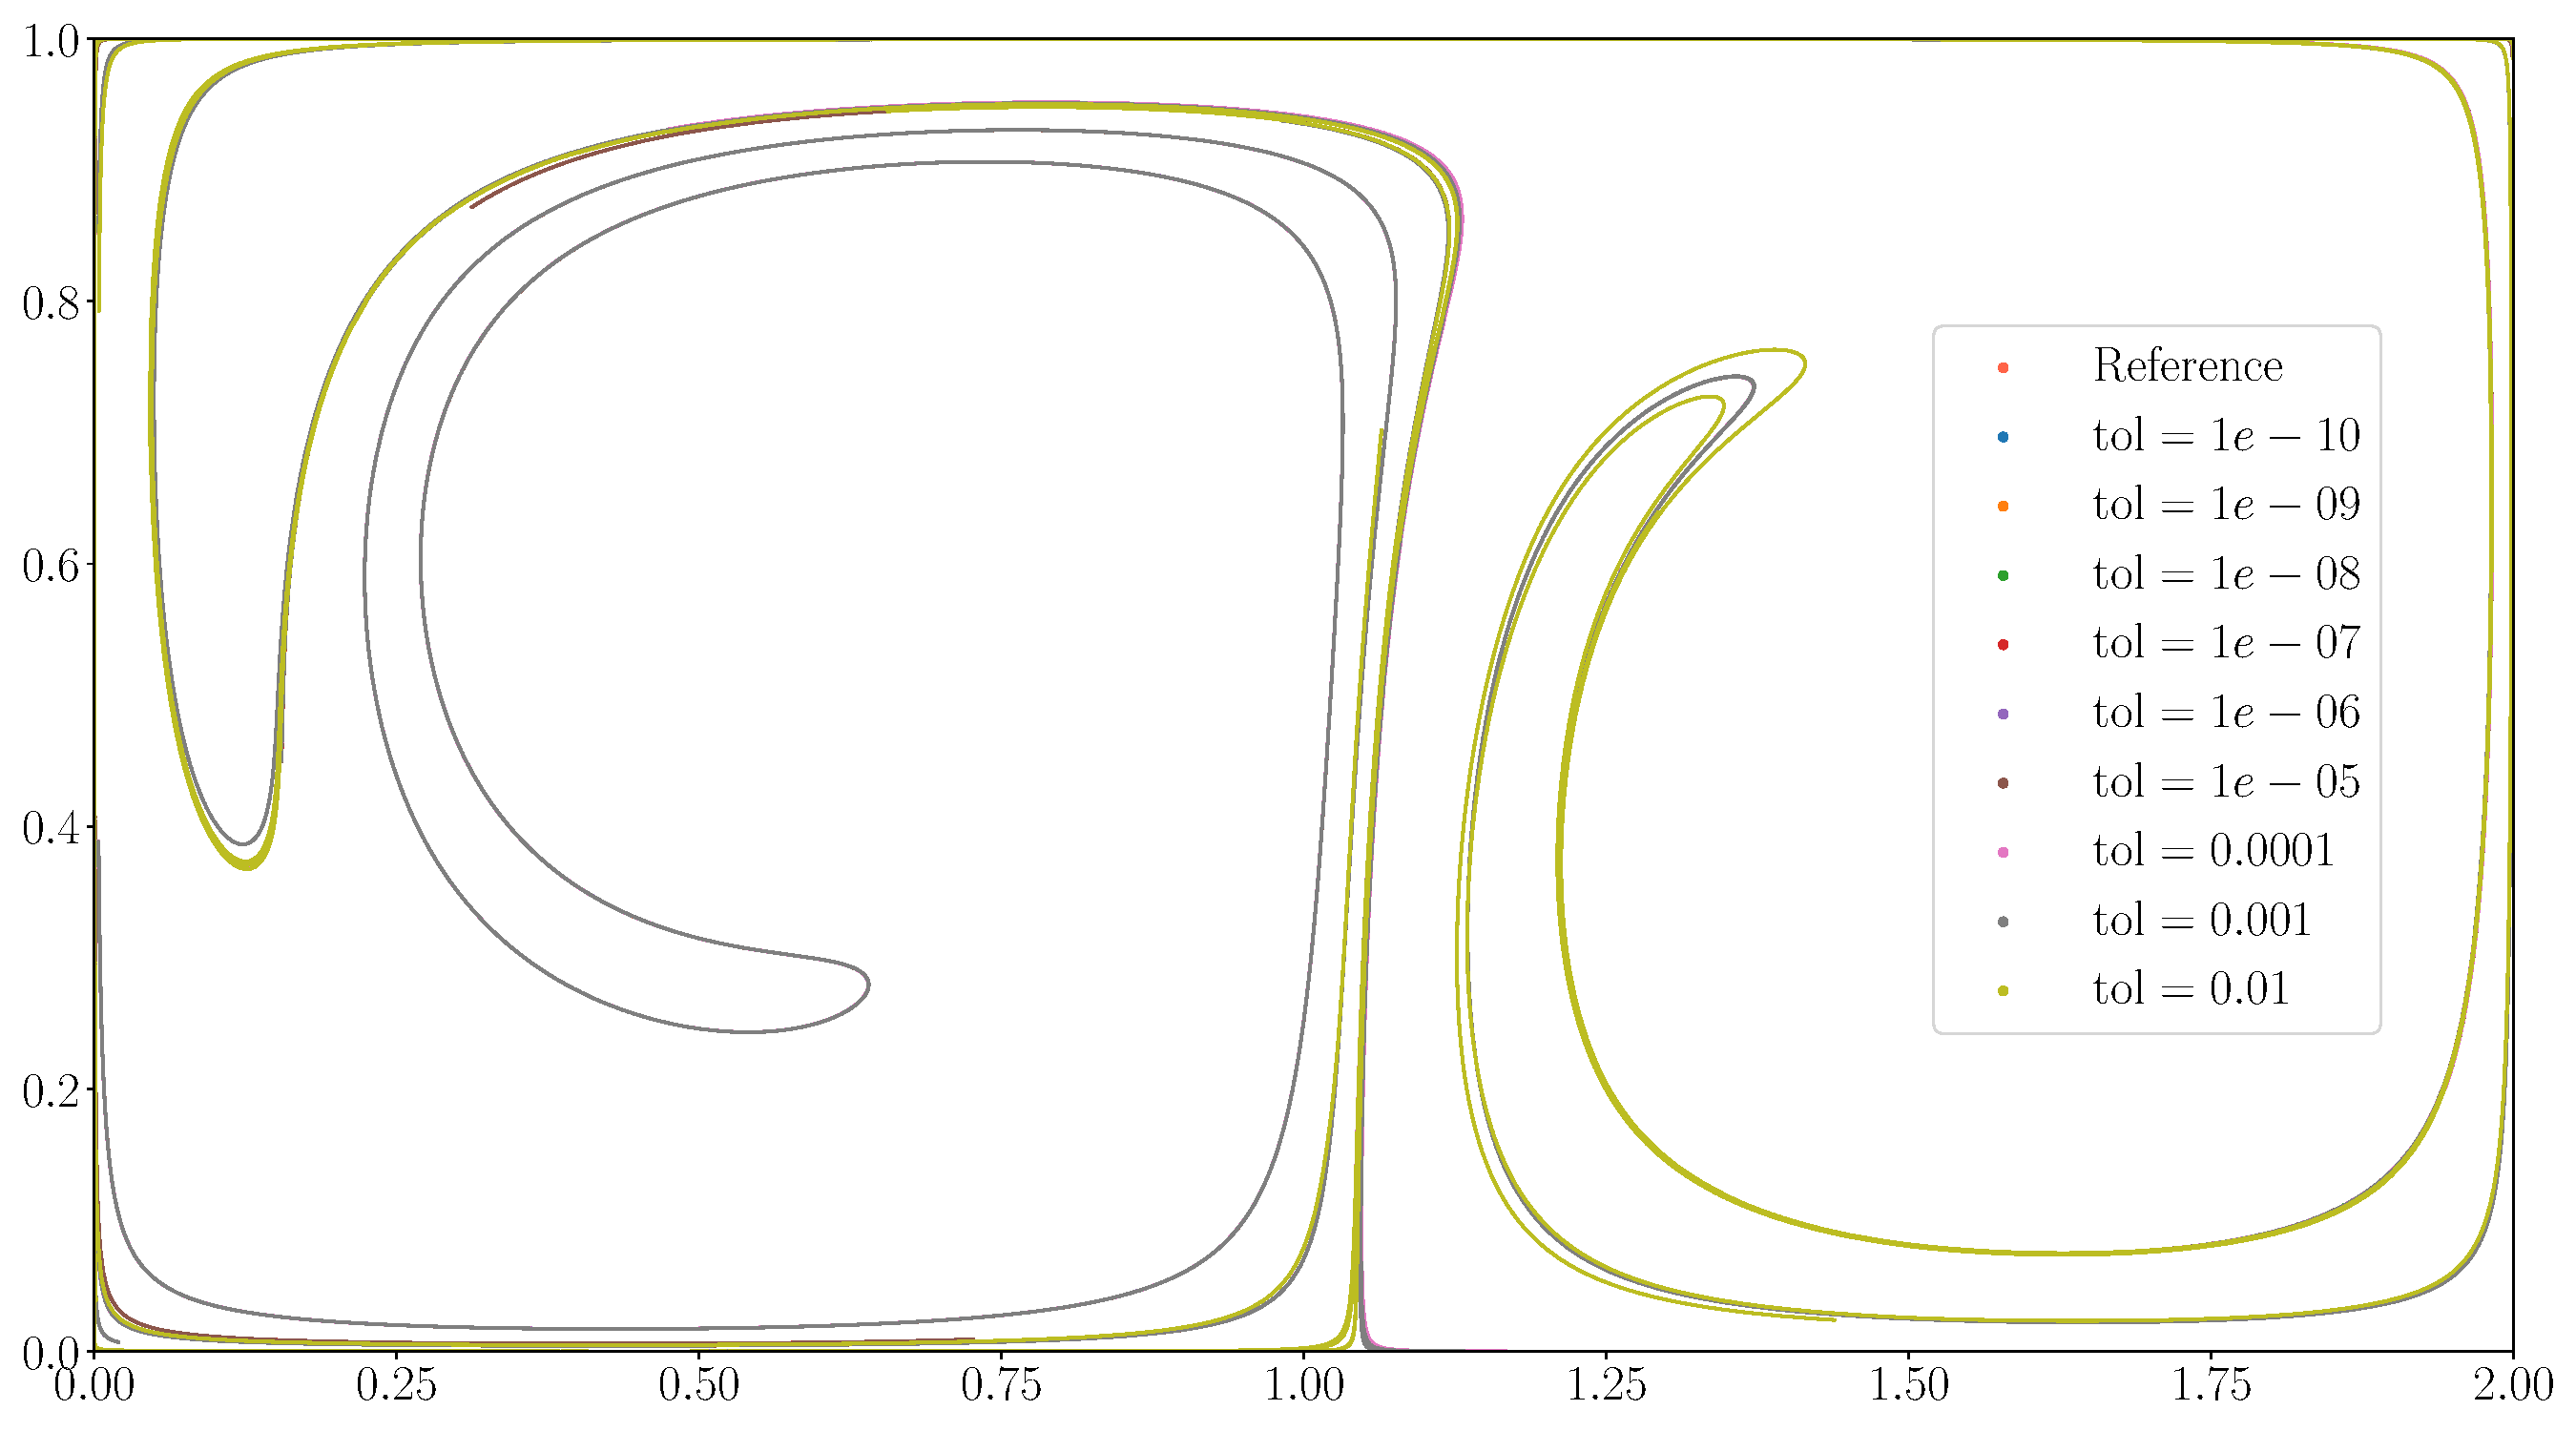
\includegraphics[width=0.9\linewidth]{figures/lcs_figures/rkdp87.pdf}
    \caption[LCS curves found by means of the Dormand-Prince 8(7) integration
    scheme]{
        LCS curves found by means of the Dormand-Prince 8(7) integration
        scheme. The reference LCS, as shown by itself in figure
        \ref{fig:referencelcs}, is plotted on the bottom layer. Note that
        the LCS for the lowest tolerance level considered, that is,
        $\textnormal{tol}=0.1$, is not included. This is because the
        corresponding $\mathcal{U}_{0}$ domain, shown in figure
        \ref{fig:u0_dp87}, and the reference $\mathcal{U}_{0}$, shown in figure
        \ref{fig:u0_domain} are unlike one another. Here, there are visible
        dissimilarities for for all tolerance levels $\textnormal{tol}>10^{-6}$,
        in particular in the lower left corner.}
    \label{fig:lcs_rkdp87}
\end{figure}
